Groco will  use a relational database to keep back end information uniform and well structured. There will be 5 different table subsystems. They are user table subsystem, meal plan table subsystem, brand table subsystem, ingredients table subsystem and recipe table subsystem.

\subsection{Layer Operating System}
The database layer will run on AWS. Thus, it will use whatever operating system AWS is using.

\subsection{Layer Software Dependencies}
The database layer will depend upon postgres for the creation of tables and execution of queries. Also, the database layer will depend upon Amazon Web Services(AWS) for hosting the database on the cloud. 

\begin{figure}[h!]
	\centering
 	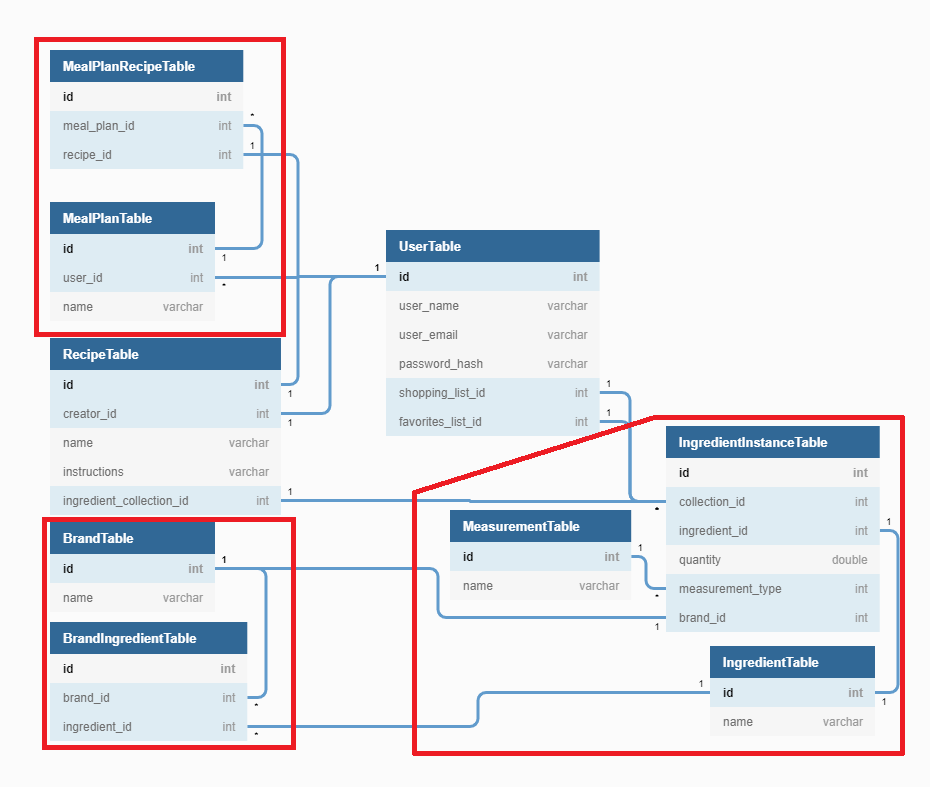
\includegraphics[width=0.60\textwidth]{images/Database.png}
 \caption{Database Diagram}
\end{figure}

\subsection{USER TABLE SUBSYSTEM }
The User table Subsystem will be used for storing identifiable information about each user and holding information to help the user. It has only one table called User table.

\begin{figure}[h!]
	\centering
 	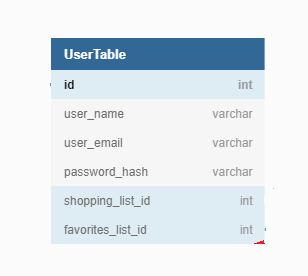
\includegraphics[width=0.60\textwidth]{images/User_Table.png}
 \caption{User Table subsystem }
\end{figure}

\subsubsection{Subsystem Software Dependencies}
User Table subsystem does not have additional dependencies.

\subsubsection{Subsystem Programming Languages}
The user table subsystem will be created using SQL and queried using SQL.

\subsubsection{Subsystem Data Processing}
Whenever a user is added to the system, their email, username, and password will be added to this table.A global ID will also be used to improve data efficiency and ensure data integrity. 

\subsection{MEAL PLAN TABLE SUBSYSTEM }
The Meal Plan Subsystem will be in charge of complying with customer requirements regarding having meal plans and related features. It has two tables called meal plan recipe table and meal plan table.

\begin{figure}[h!]
	\centering
 	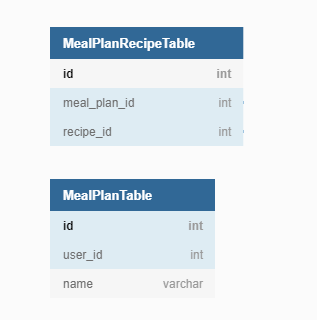
\includegraphics[width=0.60\textwidth]{images/MealPlan_SubSystem.png}
 \caption{Meal plan table subsystem diagram}
\end{figure}

\subsubsection{Subsystem Software Dependencies}
Meal plan subsystem does not have additional dependencies.

\subsubsection{Subsystem Programming Languages}
The meal plan subsystem will be created using SQL and queried using SQL.

\subsubsection{Subsystem Data Processing}
Meal plan recipe table will has mealplanid as a foreign key and it will use that foreign key when a join operation is required between meal plan recipe table and meal plan table.

\subsection{INGREDIENT TABLE SUBSYSTEM }
The Ingredients Subsystem will be used for storing ingredients required in the construction of a meal plan. This subsystem has three tables and they are called measurement table, ingredient table and ingredient instance table.

\begin{figure}[h!]
	\centering
 	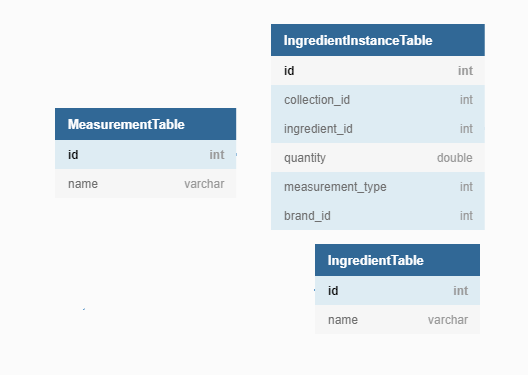
\includegraphics[width=0.60\textwidth]{images/Ingredient_SubSystempng.png}
 \caption{Ingredient Table subsystem}
\end{figure}

\subsubsection{Subsystem Software Dependencies}
Ingredient Table subsystem does not have any additional dependencies.

\subsubsection{Subsystem Programming Languages}
The user table subsystem will be created using SQL and queried using SQL.

\subsubsection{Subsystem Data Processing}
The ingredients instance table will use measurement type and ingredient id foreign keys when the join operation is required between measurement table, ingredient table and ingredient instance table.

\subsection{RECIPE TABLE SUBSYSTEM }
The Recipe Table Subsystem will responsible maintaining lists of all recipes, along with associated ingredient collection IDs. It has only one table called recipe table.

\begin{figure}[h!]
	\centering
 	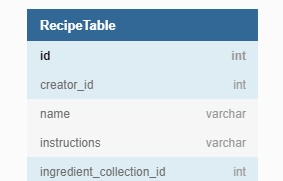
\includegraphics[width=0.60\textwidth]{images/Recepice_Subsystem.png}
 \caption{Recipe Table subsystem diagram}
\end{figure}

\subsubsection{Subsystem Software Dependencies}
Recipe Table does not have any additional dependencies.

\subsubsection{Subsystem Programming Languages}
The user table subsystem will be created using SQL and queried using SQL.


\subsection{Brand table subsystem }
The Brand Table Subsystem will responsible maintaining lists of all brands, along with associated ingredient of the brand. This subsystem has two tables: Brand Table and Brand Ingredient Table.

\begin{figure}[h!]
	\centering
 	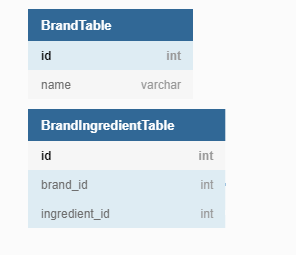
\includegraphics[width=0.60\textwidth]{images/Brand_Table.png}
 \caption{Recipe Table subsystem diagram}
\end{figure}

\subsubsection{Subsystem Software Dependencies}
Recipe Table does not have any additional dependencies.

\subsubsection{Subsystem Programming Languages}
The user table subsystem will be created using SQL and queried using SQL.

\subsubsection{Subsystem Data Processing}
Brand ingredient table has brandId as foreing key and it will be used when a join operation is required between brand table and brand ingredient table. It also has ingredient id as a foreign key which will be used when a join operation is required between brand ingredient table and ingredient table.